\documentclass[a4paper,11pt,italian]{article}
\usepackage[T1]{fontenc}
\usepackage[utf8]{inputenc}
\usepackage[italian]{babel}
\usepackage{amsmath}
\usepackage{mathrsfs}
\usepackage{hyperref}

%%%--- impostazioni font
\usepackage{sansmathfonts}
\usepackage[scaled=0.85]{helvet}
\renewcommand{\rmdefault}{\sfdefault}
\usepackage[font=footnotesize,width=.75\textwidth]{caption}

%%%--- frazioni carine \sfrac{}{}
\usepackage{xfrac}

%%%--- interlinea
\usepackage{setspace}
\setstretch{1.3}

%%%--- multicolonna
\usepackage{multicol}

%%%--- figure in orizzontale
\usepackage{rotating}

%%%--- margini e bordo
\usepackage[margin=2.7cm]{geometry}
% \usepackage{showframe}

%%%--- impostazioni tikz e grafici
\usepackage{pgf,tikz,pgfplots,bm,pgf-spectra,graphicx,timelines}
\usepackage{circuitikz}
\usetikzlibrary{angles,quotes,arrows,shapes,decorations.markings}
\tikzset{fleche/.style args={#1:#2}{postaction=decorate,decoration={name=markings,mark=at position #1 with {\arrow[#2,scale=1.5]{latex}}},},}
\pgfplotsset{compat=1.15}
\usepgfplotslibrary{units,fillbetween}

%%%--- info documento
\title{\textbf{\Huge \color{colorSitoScuro}Formulario di Fisica}}
\author{\LARGE \color{colorSitoScuro}Mattia Cozzi}
\date{\large \color{colorSitoChiaro}\href{http://mattiacozzi.altervista.org/}{mattiacozzi.altervista.org}}

%%%--- riferimenti intelligenti
\usepackage[noabbrev]{cleveref} %opzione capitalize per tutto maiuscolo

%%%---righelli migliori per tabelle
\usepackage{booktabs}

%%%--- impostazioni dei colori
\usepackage{xcolor}
\usepackage{sectsty}
\usepackage{enumitem}
%%%--- TEAL
\definecolor{colorSito}{rgb}{.04,.212,.22}
\definecolor{colorSitoChiaro}{rgb}{.20,.408,.416}
\definecolor{colorSitoScuro}{rgb}{.0,.133,.141}
%%%--- BORDEAUX
% \definecolor{colorSito}{rgb}{.612,.067,.192}
% \definecolor{colorSitoChiaro}{rgb}{.69,.145,.271}
% \definecolor{colorSitoScuro}{rgb}{.22,.0,.0}

\sectionfont{\color{colorSito}}  %imposta il colore delle sezioni
\subsectionfont{\color{colorSitoChiaro}}  %imposta il colore delle sottosezioni
\subsubsectionfont{\color{colorSitoChiaro}}  %imposta il colore delle sottosottosezioni
\setlist[description]{format=\textcolor{colorSitoScuro}} %imposta il colore degli elementi di una lista di definizione

%%%--- nuovi comandi


%%%---cerca NON NECESSARIO per trovare le formule commentate
\begin{document}




\begin{description}
  
  \item[Curve sperimentali per l'emissione di energia a diverse temperature]
  Nella \Cref{img:radianza} la zona evidenziata indica lo spettro della luce visibile; alla sua sinistra la radiazione ultravioletta, alla sue destra i raggi infrarossi.
  La previsione classica è data dalla legge di Rayleigh-Jeans.
 
% \begin{figure}[htb]\centering
% 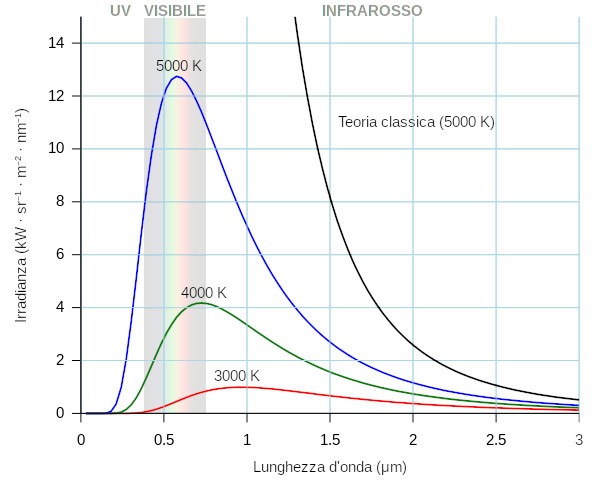
\includegraphics[width=.7\columnwidth]{parts/corponero.jpg}
% \caption{Dati sperimentali per la quantità di energia emessa nelle diverse lunghezze d'onda. L'area sottesa dalla curva fornisce l'energia totale emessa.}
% \label{img:radianza}
% \end{figure}
 
\begin{figure}[htpb]\centering
  \begin{tikzpicture}[samples=700, scale=1.2]
  \begin{axis}[
    xmin=0.1,
    xmax=4,
    xlabel={{\footnotesize $\lambda \, [nm]$}},
    ymin=0,
    ymax=.3,
    ylabel={{\footnotesize $\rho (\lambda; T) \, [\sfrac{W}{m^2}]$}},
    xtick=\empty,
    ytick=\empty,
    no markers,
    grid=both,domain=0.1:40,
    style={}]
     \fill [black!10] (.5,0.001) rectangle (1,pi-0.001);
     \addplot[fill=colorSitoScuro,fill opacity=.25,thick,colorSitoScuro,smooth] {(8)/((x^5)*(exp((3.6)/(x))-1))};
     \addlegendentryexpanded{{\footnotesize $T = 5000 \, K$}}
     \addplot[fill=colorSito,fill opacity=.25,thick,colorSito,smooth] {(8)/((x^5)*(exp((4.3)/(x))-1))};
     \addlegendentryexpanded{{\footnotesize $T = 4000 \, K$}}
     \addplot[fill=colorSitoChiaro,fill opacity=.25,thick,colorSitoChiaro,smooth] {(8)/((x^5)*(exp((5.3)/(x))-1))};
     \addlegendentryexpanded{{\footnotesize $T = 3000 \, K$}}
     \addplot[thick,colorSitoChiaro!60,dashed,domain=.5:4] {(1/((4*(x-.4)^2)))};
     \addlegendentryexpanded{{\footnotesize previsione classica}}
     \draw[black!30] (.5,0.0001)--(.5,.3-0.0001);
     \draw[black!30] (1,0.0001)--(1,.3-0.0001);
     \node[below] at (.75,.3) {{\scriptsize visibile}};
     \node[below] at (.3,.3) {{\scriptsize UV}};
     \node[below] at (1.15,.3) {{\scriptsize IR}};
  \end{axis}
  \end{tikzpicture}
\caption{Dati sperimentali per la quantità di energia emessa nelle diverse lunghezze d'onda. L'area sottesa dalla curva fornisce l'energia totale emessa.}
\label{img:radianza}
\end{figure}
  
\end{description}

\end{document}
